\documentclass[../Draft_harmonization_paper.tex]{subfiles}
% \documentclass{article}
% \usepackage[utf8]{inputenc}
% \usepackage{hyperref}
% \usepackage{float}
% \usepackage[table,xcdraw]{xcolor}
% \usepackage{color, colortbl}
% \usepackage{longtable}
% %\usepackage[sort&compress,square,comma,authoryear]{natbib}
% \usepackage{booktabs}
% \usepackage{graphicx}
% \graphicspath{{/home/kunz/Dokumente/Projects/Trait_DB/Invertebrate_traits/Paper/Figures/}}
% \usepackage{longtable}
% \usepackage{rotating}
% \usepackage{geometry}
% \usepackage{array}

% \definecolor{Gray}{gray}{0.9}

% \newcommand{\specialcell}[2][c]{%
%   \begin{tabular}[#1]{@{}c@{}}#2\end{tabular}}

\begin{document}
%! Trait (species) scores along segments of river

\subsection*{Re-analysis of Szöcs et al. using harmonized and aggregated grouping features}

Overall, using the harmonized grouping features led to only slightly different results in comparison to the original analysis (Figure \ref{fig:rda_species_scores} and SI). According to the RDA of the trait composition, sites with high salinity were characterized by families that possess the traits multivoltinism, ovoviviparity, gill-respiration, and feeding mode shredder. Only families with the trait life cycle duration $> 1$ year failed to characterize sites with high salinization. Also, life cycle duration $<= 1$ year did not characterise sites not impacted by salinity. Like in the original analysis, transition and upstream sites from the point source were characterised by univoltine taxa and taxa that lay their eggs in aquatic environments. We also constructed the linear models of the original analyses, using the traits on the extremes of the conductivity axis and found results similar to the original analyses (Table S\ref{stab:linear_models_new} and S\ref{stab:linear_models_edi}).

For every aggregation method compared, using at family-level aggregated traits did only slightly change the species scores compared to not aggregated traits (Figure \ref{fig:rda_species_scores}). 

\begin{figure}[H]
    \label{fig:rda_species_scores}
    \centering
    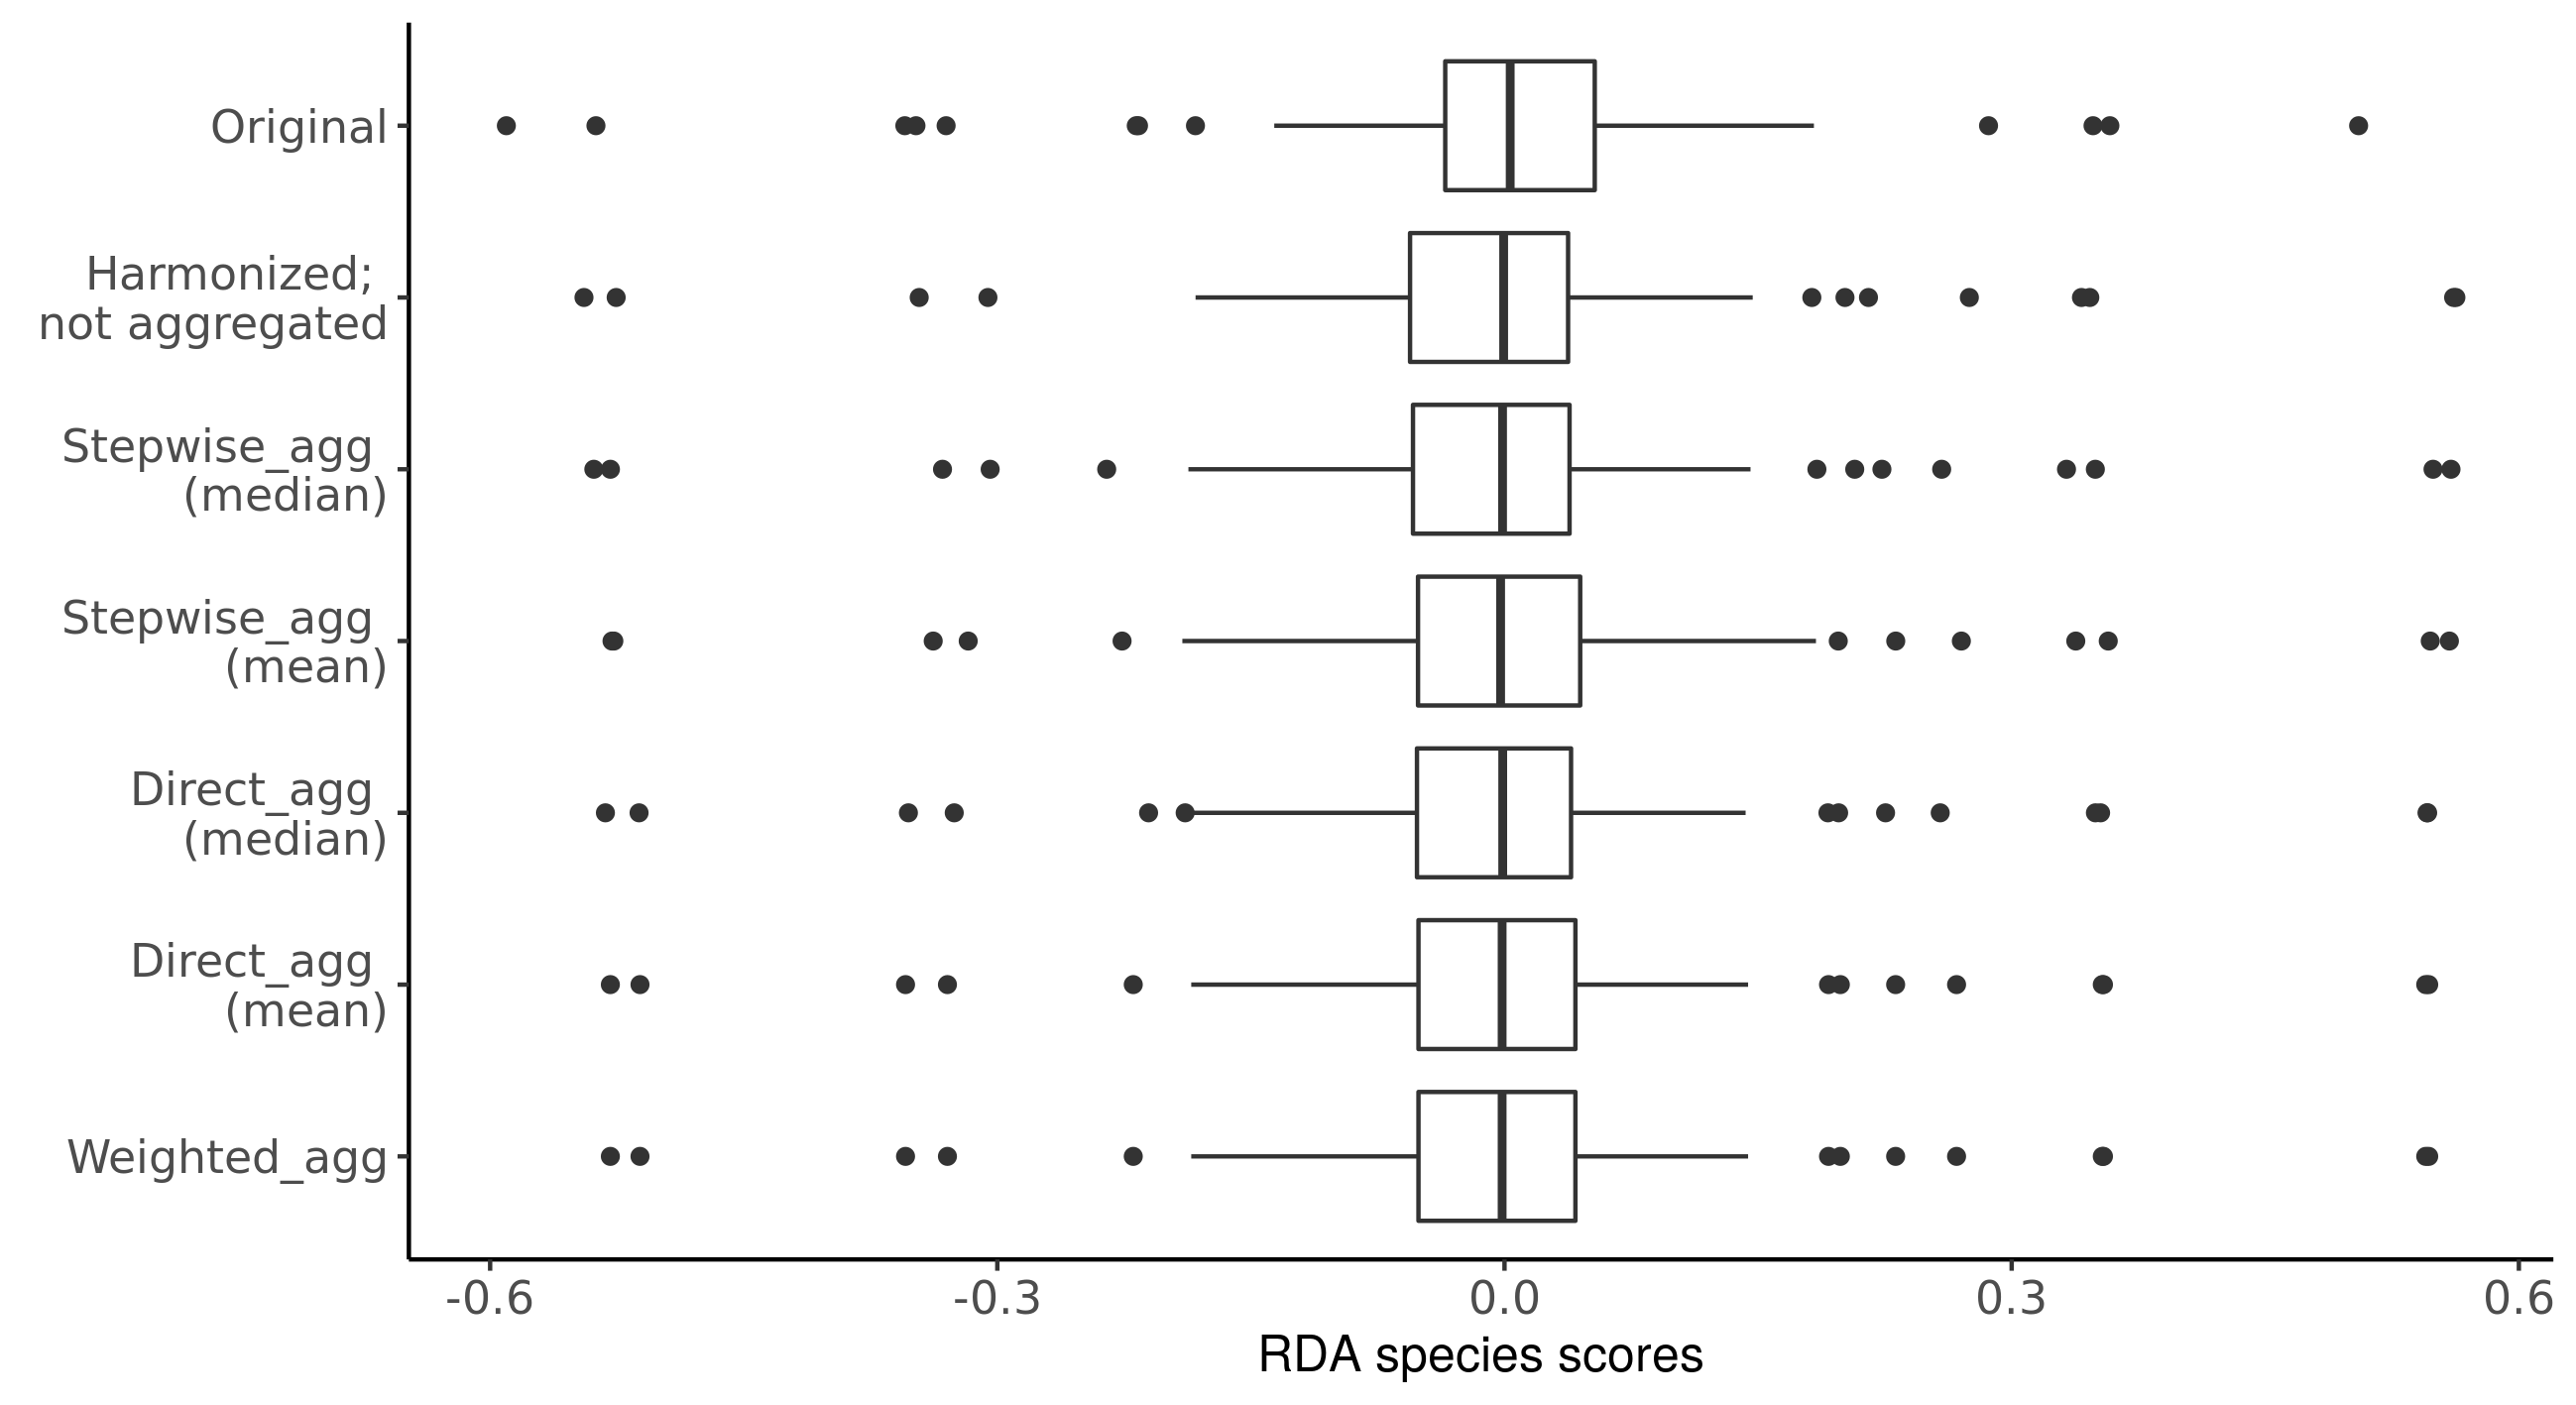
\includegraphics[width=16.5cm, height=10cm]{Species_scores_rda.png}
    \caption{Species scores obtained by RDA from the original analysis \cite{szocs_effects_2014}, using harmonized grouping features, and using harmonized grouping features with assigned trait affinities aggregated to family-level.}
    \label{fig:rda_species_scores}
\end{figure}

\end{document}